% Part I > Community response: how the field reacted, and the problems each
% response exposes. Leads into section 12 (what formalization fixes).
% Facts and sources: research/03 (publishing), 05 (applied voices), 06
% (AcadMathSci report review). Corpus statistics: eda.py on data/dataset.csv.
\section{Community response}

% [1.5 min] The field agrees AI works; it disagrees about consequences.
% Statistics recomputed 2026-11-10 from data/dataset.csv with eda.py's filters
% (152 posts in the analysis set; 141 address capability). LLM-scored,
% self-selected corpus: illustration, not a survey.
% 49% = 75 of 152 with rubric 'overall' < 0 (10 at 0, 67 positive).
\begin{frame}{Proofs and Prompts: A Sentiment Analysis}
  \centering
  \begin{tikzpicture}[x=1cm, y=1cm]
    \useasboundingbox (0,0) rectangle (14.3,-6.3);
    \node[collagecard, anchor=north west] at (0,0)
      {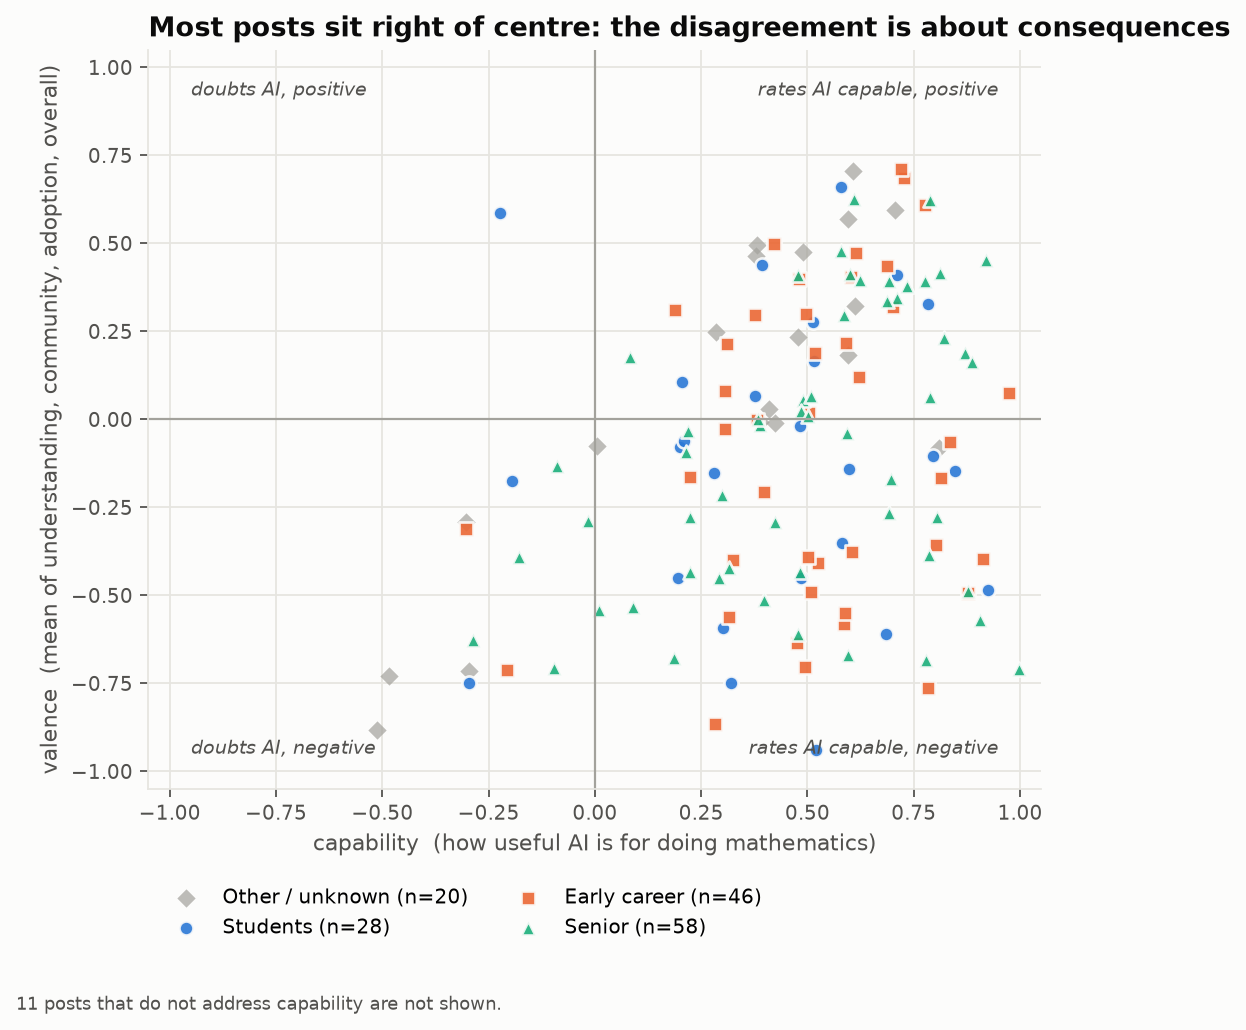
\includegraphics[height=6.1cm]{../figures/04_capability_vs_valence.png}};
    \node[anchor=north west, text width=6.2cm, align=flush left, inner sep=0pt,
          font=\sffamily\small] at (8.1,-0.35) {%
      {\color{black!55}\scriptsize 152 essays on \emph{proofsandprompts.com}, each scored by an LLM}\par\bigskip
      {\fontsize{22}{24}\selectfont\bfseries\color{tlBlue}89\%}\par
      rate AI as capable of doing mathematics\par\bigskip
      {\fontsize{22}{24}\selectfont\bfseries\color{tlOrange}49\%}\par
      view AI as a negative force overall\par\bigskip
      \textbf{The field agrees that it works.\\ It disagrees about the consequences.}};
  \end{tikzpicture}
  \slidesources{Proofs \& Prompts corpus (proofsandprompts.com), scored with Claude; analysis set of 152 posts, 141 addressing capability. Self-selected essays: an illustration, not a survey}
\end{frame}

% [1 min] The three clusters and the words that distinguish them. The method
% is kept off the slide (removed 2026-11-10); it is here for questions.
% Method (cluster.py, reviewed 2026-11-10): an LLM embeds each post in an
% interpretable semantic space (rubric.py: seven scored dimensions). Clustering
% uses two coordinates of that embedding, capability and valence (mean of
% understanding, community, adoption, overall), standardised, with k-means (k=3, 141 posts; silhouette 0.43, bootstrap ARI median 0.91).
% Cluster names come from a rule on the centres (name_cluster: capability >= 0.4
% -> "capable", else "doubted"; valence > 0.15 positive, < -0.15 negative). The
% "doubted" centre sits at capability +0.04, i.e. neutral rather than doubting.
% Word clouds are computed afterwards from the raw text: per-cluster log-odds of a term appearing in a post
% (z >= 2, >= 5 posts), with a hand-curated list of generic words removed.
\begin{frame}{Proofs and Prompts: What Each Cluster Writes About}
  \centering
  \begin{tikzpicture}[x=1cm, y=1cm]
    \useasboundingbox (0,0) rectangle (14.3,-5.95);
    % clusters in the score plane (figure is 0.872 wide per unit height: ~5.1 cm here);
    % cluster names, sizes and centres are labelled inside the figure
    \node[collagecard, anchor=north west] at (0,0)
      {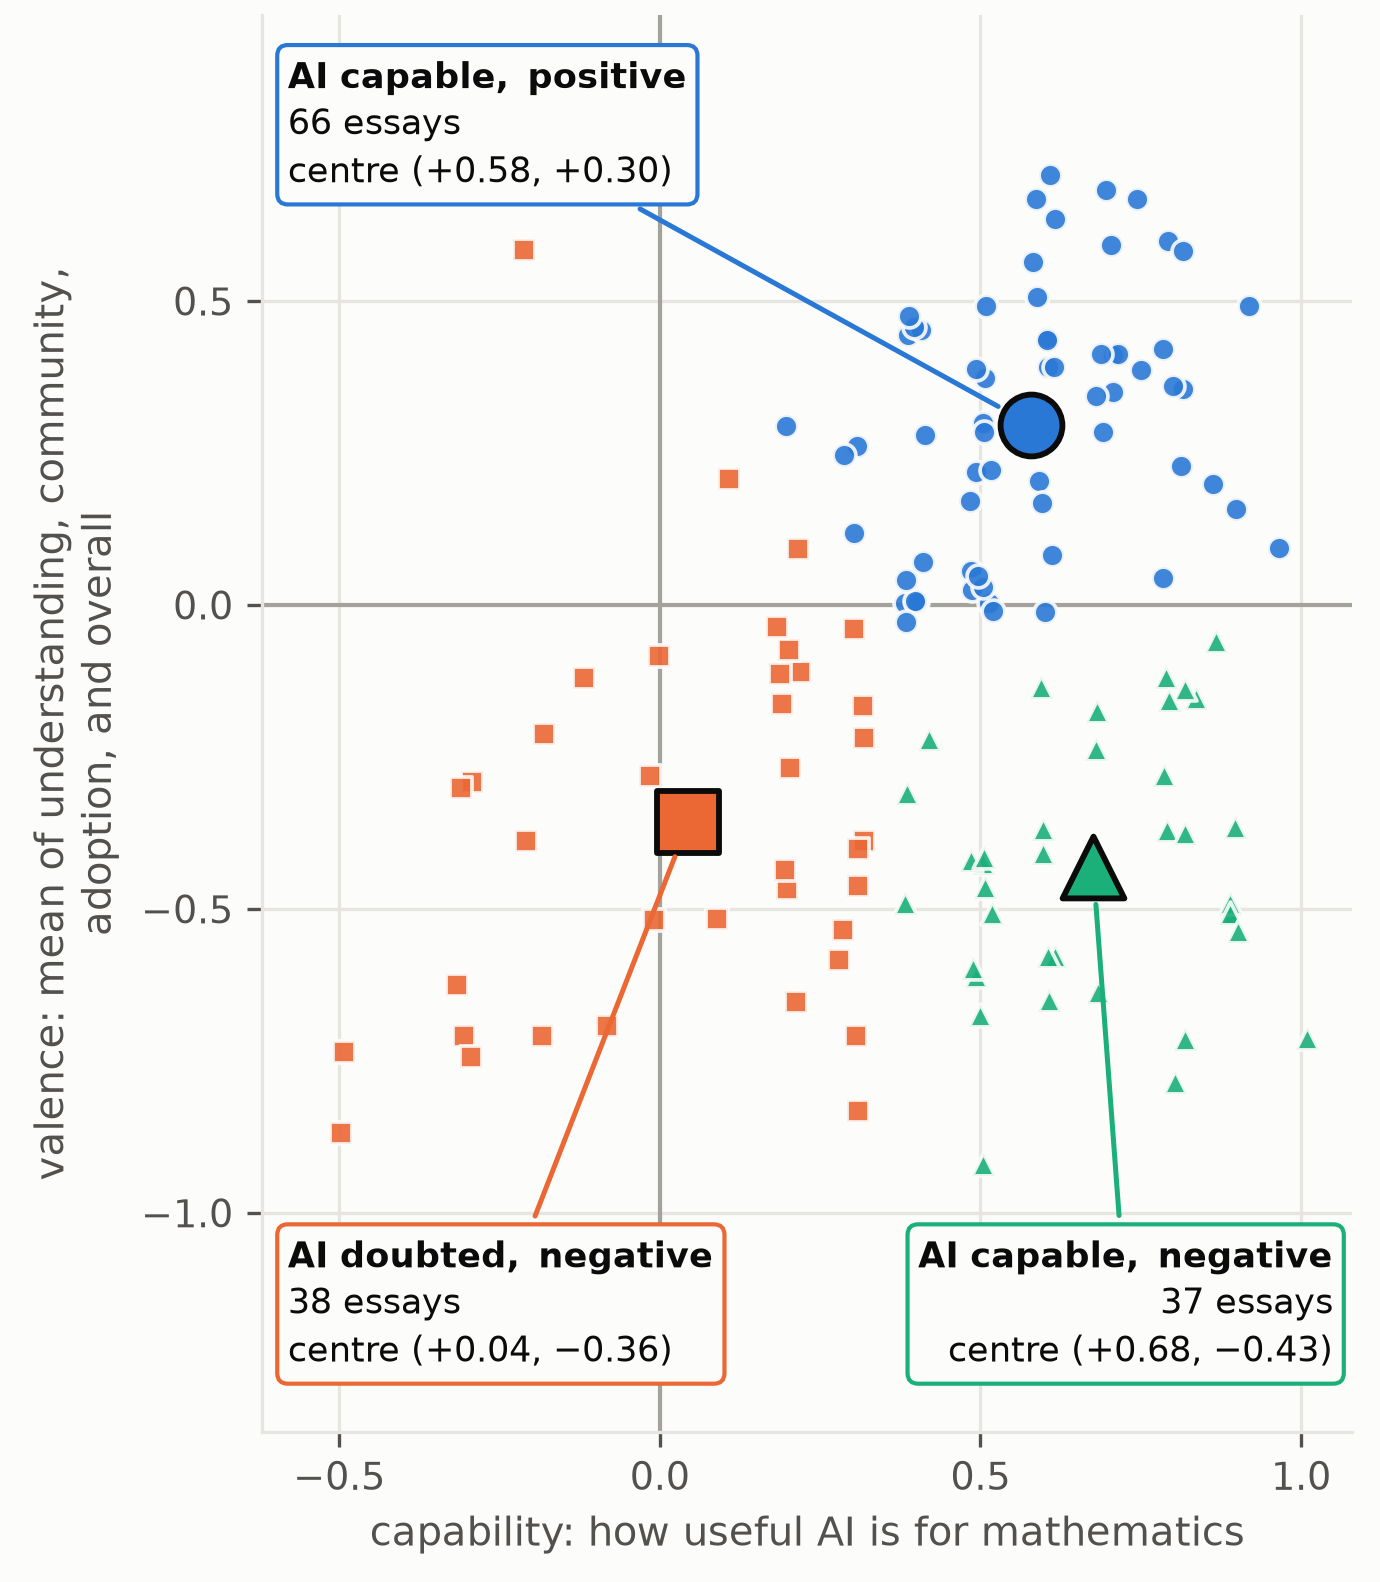
\includegraphics[height=5.85cm]{../figures/08_clusters.png}};
    % word clouds, one per cluster, stacked top to bottom in the same colours (2:3 figure)
    \node[collagecard, anchor=north east] at (14.3,0)
      {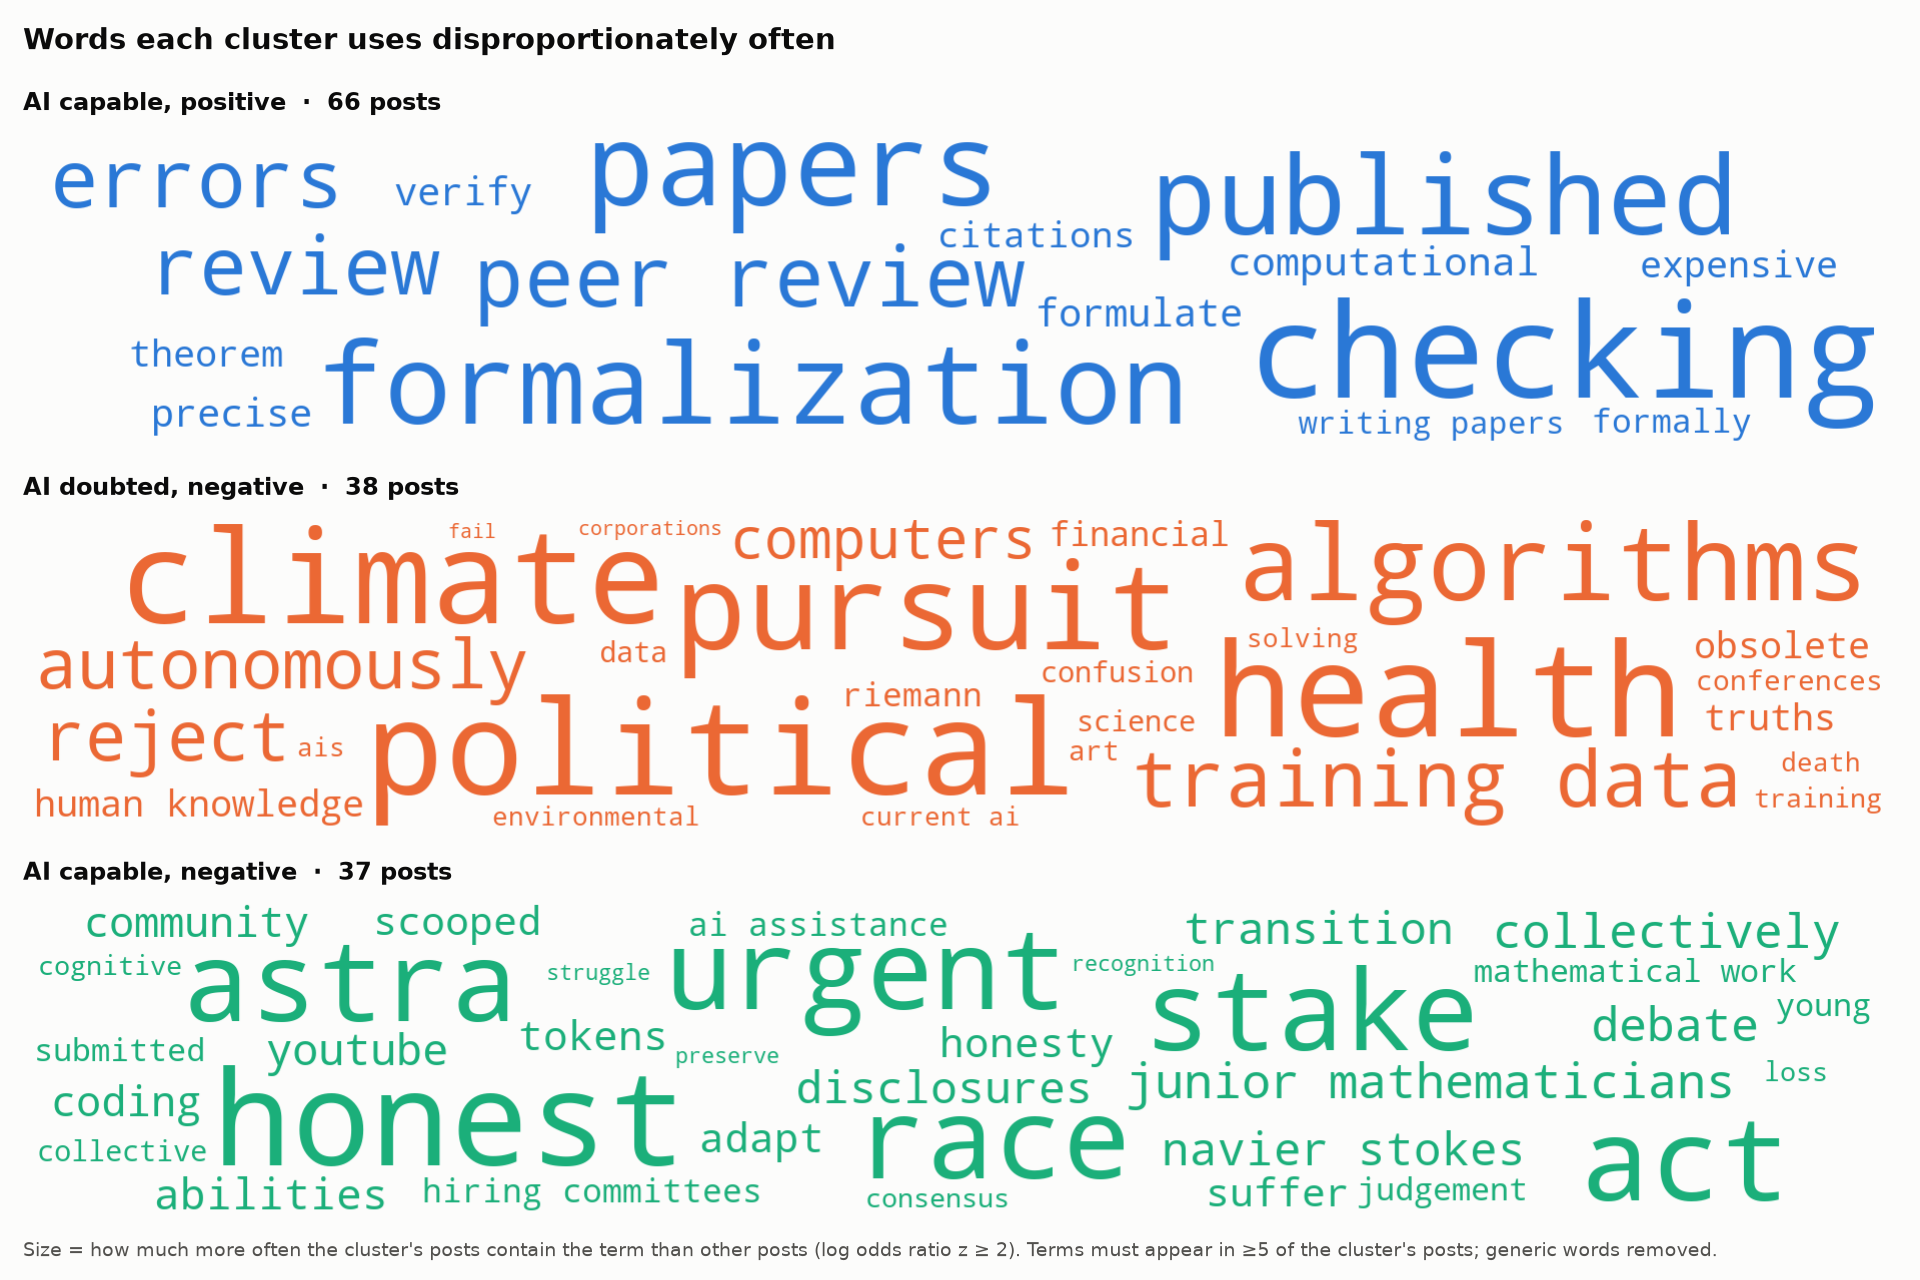
\includegraphics[height=5.85cm]{../figures/09_wordclouds.png}};
  \end{tikzpicture}
  \slidesources{Proofs \& Prompts corpus; scores from Claude (rubric.py); clustering and word statistics from cluster.py. Self-selected essays: an illustration, not a survey}
\end{frame}

% [2 min] Who did what, and who is told. Each row: the problem, the case that
% exposed it, the institutional response, and how far that response reaches.
\begin{frame}{Credit, disclosure and confidentiality}
  \footnotesize\sffamily
  \renewcommand{\arraystretch}{1.35}
  \begin{tabularx}{\linewidth}{@{}p{2.3cm}YYp{1.5cm}@{}}
    \toprule
    \tabhead{Problem} & \tabhead{Case} & \tabhead{Response} & \tabhead{Status}\\
    \midrule
    \rowhead{Credit} & AI reuses known ideas without attribution: 8 of Aletheia's 13 meaningful Erd\H{o}s results were already in the literature. Kolda: ``Human--AI scrapple''
      & Leiden Declaration (Jun 2026, endorsed by the IMU): human responsibility, attribution & \stpartial\\
    \rowhead{Priority} & Navier--Stokes priority dispute (C\'ordoba \& Mart\'inez-Zoroa; Buckmaster \& Alp\"oge)
      & AGMAI release guidelines (29 Sep): review before announcement, release prompts. Labs withheld prompts & \stopen\\
    \rowhead{Disclosure} & 1 in 6 math preprints read as AI-written without saying so. At ICML 2026, 22.5\% of reviewers used an LLM under a ban
      & Disclosure statements (arXiv, Springer, Leiden); SIAM AI policy v2.0 & \stpartial\\
    \rowhead{Confidentiality} & Referees uploading manuscripts to AI tools
      & LMS: misconduct. SIAM v2.0: ``non-delegation of scholarly judgement'' & \stpartial\\
    \bottomrule
  \end{tabularx}\par\medskip
  {\color{black!60}\scriptsize The rules already bind individuals; none of them can be checked from the paper alone.}
  \slidesources{Reisinger et al., AcadMathSci, Oct 2026 (A.3, C.1, C.4, C.5) \textbullet{} Kolda, Silicon Reckoner, Feb 2026 \textbullet{} Martin, Nov 2026 \textbullet{} Kim et al., arXiv 2609.19420}
\end{frame}

% [1.5 min] Volume against fixed refereeing capacity.
\begin{frame}{Review capacity}
  \footnotesize\sffamily
  \renewcommand{\arraystretch}{1.35}
  \begin{tabularx}{\linewidth}{@{}p{2.3cm}YYp{1.5cm}@{}}
    \toprule
    \tabhead{Problem} & \tabhead{Case} & \tabhead{Response} & \tabhead{Status}\\
    \midrule
    \rowhead{Volume} & arXiv math: 7,428 submissions in Sep 2026, against 4,252 a year earlier (+75\%). A few prolific authors drive much of it
      & arXiv: two new submissions per submitter per month (1 Oct). STOC 2027: at most five per author & \stdone\\
    \rowhead{Referees} & Six probability journals paused new submissions (19 Oct\,--\,8 Nov). Editors report they cannot find a referee
      & Pauses; proposals for paid, AI-assisted refereeing (Maltsev) & \stopen\\
    \rowhead{AI reviewing} & ICLR 2026: 21\% of reviews fully AI-generated
      & ICLR plans automated screening of reviews and submissions & \stpartial\\
    \rowhead{Bypassed review} & Results announced on X and GitHub before any review (Navier--Stokes; 719 manuscripts in a day)
      & Leiden and AGMAI: announce through peer review. Palomar registry of Lean-verified results (18 Aug); a proposed journal requiring Lean proofs (Guo, 17 Oct) & \stpartial\\
    \bottomrule
  \end{tabularx}\par\medskip
  {\color{black!60}\scriptsize Restricting and disclosing are in place; verifying is the structural response, and it is still a prototype.}
  \slidesources{AcadMathSci, Oct 2026 (\S1.2) \textbullet{} Nee, Zhong \& Ni, arXiv 2609.04872 \textbullet{} Fortnow, Sep 2026 \textbullet{} Pangram, ICLR 2026 (self-reported) \textbullet{} Tao, blog, 18 Aug and 17 Oct 2026}
\end{frame}

% [1.5 min] Who learns, who can afford it, and what gets studied.
\begin{frame}{Training, access and narrowing}
  \footnotesize\sffamily
  \renewcommand{\arraystretch}{1.35}
  \begin{tabularx}{\linewidth}{@{}p{2.3cm}YYp{1.5cm}@{}}
    \toprule
    \tabhead{Problem} & \tabhead{Case} & \tabhead{Response} & \tabhead{Status}\\
    \midrule
    \rowhead{Training} & Students given unrestricted GPT-4 scored 17\% lower once access was removed; a tutor with guardrails largely avoided the harm (Bastani et al.)
      & Vivas and in-person exams; AI-permitted work graded on formulation and validation & \stpartial\\
    \rowhead{Access} & Only 11\% of researchers have institutional funding for their main AI tool (Springer Nature, 10,480 researchers). Navier--Stokes cost an estimated \pounds4.9M
      & Token costs eligible on grants (proposed); SAIR Open Math OS: free open models for academics & \stpartial\\
    \rowhead{Narrowing} & AI adoption shrinks topic range by 4.6\% and engagement by 22\% (Hao et al., 41M papers). Agendas drift toward ``problems easily amenable to current AI''
      & Reward understanding and long-term contribution over volume (AcadMathSci) & \stopen\\
    \bottomrule
  \end{tabularx}
  \slidesources{Reisinger et al., AcadMathSci, Oct 2026 (\S1.6, \S3.2, \S3.3, \S4.3, B.1) \textbullet{} Bastani et al., PNAS \textbullet{} Hao et al., arXiv 2412.07727}
\end{frame}
